\chapter[Electromechanical Design]{Electromechanical Design\footnote{Part of the electromechanical design work in this chapter was completed as part of the ECE 499 project course at the University of Waterloo.}} % (fold)
\label{cha:design}

This chapter presents the electromechanical design of a bipedal robot for experimental validation. Each leg is selected to have 7 DOF (breakdown provided in Table~\ref{tab:doftable}) to enable a wide range of motion for balancing and walking. This provides a total of 14 actuated DOF for the bipedal robot. A serial link mechanism approach is used for its simplicity in design and kinematics. The bipedal robot is a fully powered active walker (i.e. every joint is actively controlled) with an electric motor drivetrain. DC motors with geared drives are selected because it is easy to model the actuator dynamics and achieve accurate joint level position control. 

\begin{table}[h]
  \centering
  \caption{Degrees-of-Freedom in each leg of the bipedal robot.}
    \begin{tabular}{rc}
    \addlinespace
    \toprule
    \textbf{Joint} & \textbf{DOF} \\
    \midrule
    Hip   & 3 \\
    Knee  & 1 \\
    Ankle & 3 \\
    \bottomrule
    \end{tabular}
  \label{tab:doftable}
\end{table}

There are several other key design considerations which impact the performance of the finished product. The complete design process consisted of selecting the appropriate drivetrain components and designing the mechanical chassis. The primary design objective was to produce enough mechanical power for the robot to achieve walking. The secondary design objective was to keep the overall weight low and raise center-of-mass (COM) position as high as possible. 

The initial design specification was obtained by modeling the system dynamics during an estimated gait cycle (Section~\ref{sec:designspec}). The selection of electromechanical components comprising the drivetrain system was used to address the primary design objective (Section~\ref{sec:drivetrain}). These drivetrain components include DC motors and appropriate gearing to provide the reduction ratio required to meet the initial design specifications. After the primary objective was addressed and the drivetrain components were selected, the secondary design objectives were satisfied by adjusting the mechanical structure and manipulating placement of components (Section~\ref{sec:chassis}).

%======================================================================
%   D Y N A M I C  M O D E L I N G
%======================================================================

\section{Dynamic Modeling} % (fold)
\label{sec:designspec}

A dynamic model of the proposed system must be developed and analyzed under normal operating conditions to determine the forces acting on the system and torques experienced at each of the joints. The forward or direct dynamic model provides a transformation from the joint torques ($\vtau$) to the resulting joint positions ($\q$), velocities ($\vec{\dot{q}}$) and accelerations ($\vec{\ddot{q}}$).

\begin{equation}
	\ddq = f(\vtau, \q, \dq, \F{C})
\end{equation}

$\F{C}$ represents the contact force(s) felt at the feet. Given this model, a dynamic simulation environment can be designed to estimate the torque loading at different joints on the bipedal robot during the gait cycle. This estimate can form the basis of the initial design specifications from which motors and gearing can be selected. An important consideration in this model is the inclusion of contact forces during the stance phase of the gait cycle. The ground reaction forces exerted on the robot's feet have a significant impact on the dynamic requirements of each joint.
% section overview (end)

\subsection{Equations of Motion} % (fold)
\label{sec:forward_dynamics}

The general form of the equation of motion describing a $n$-DOF humanoid robot (with a floating base) is given by: 

\begin{equation}
	\label{eq:eom1}
	\inertia \ddq + \coriolis \dq + \gravity = \vtau + \Jt{} \F{C}
\end{equation}

Where $\inertia$ is the $(n+6) \times (n+6)$ inertia matrix, $\coriolis$ are the centripetal/Coriolis terms, $\gravity$ is the gravity vector and $\J{}{}$ is the Jacobian matrix which provides the mapping between the joint and work space variables. The $(n+6) \times 1$ generalized force vector $\vtau$ is segmented as follows:

\begin{equation}
	\label{eq:gentau}
	\vtau = {\begin{bmatrix} {\vtau}_{\mathbf{act}} & {\vtau}_{\mathbf{base}} \\ \end{bmatrix}}^T
\end{equation}

Where ${\vtau}_{\mathbf{act}}$ represents the $n$ actuated DOF and ${\vtau}_{\mathbf{base}} = \bf{0}_{6 \times 1} $ are the remaining non-actuated DOF at the floating base. In order to incorporate the effects of contact forces at both feet of the biped robot, (\ref{eq:eom1}) is expanded as follows: 

\begin{equation}
	\label{eq:eom2}
	\begin{bmatrix} \mathbf{A_{11}} & \mathbf{A_{12}} \\ \mathbf{A_{21}} & \mathbf{A_{22}} \end{bmatrix} 
	\begin{bmatrix} \ddq_{\mathbf{act}} \\ \ddq_{\mathbf{base}} \end{bmatrix} + 
	\begin{bmatrix} \vec{b}_{\mathbf 1} \\ \vec{b}_{\mathbf 2} \end{bmatrix} = 
	\begin{bmatrix} {\vtau}_{\mathbf{act}} \\ \mathbf{0} \end{bmatrix} + 
    \Jt{L}\F{L} + \Jt{R}\F{R}
\end{equation}

Where the generalized acceleration vector $\ddq_{\mathbf{act}}$ represents the $n$-DOF joint motion and $\ddq_{\mathbf{base}}$ represents the 6 DOF base motion. The gravitational and Coriolis terms are combined into the $\vec{b}$ vector. The $\J{L}{}$ and $\J{R}{}$ are 6 x $n$ Jacobian matrices for the left and right legs, respectively. The force vectors $\F{L}$ and $\F{R}$ represent the contact force felt at the left and right foot, respectively. The method of calculating the magnitude of the force itself depends on the contact model used for the system. Equation (\ref{eq:eom2}) is used to represent the dynamics of the 14 DOF bipedal robot with $n = 14 + 6 = 20$ generalized coordinates.
% section forward_dynamics (end)

\subsection{Recursive Newton-Euler} % (fold)
\label{sec:kajita_s_matlab_toolbox}

The Recursive Newton-Euler (RNE) algorithm computes the inverse dynamics model recursively in order to arrive at a final solution for the direct dynamics \cite{Perrin:1997wn}. The algorithm serially traverses through the kinematic chain to perform calculations using Newtonian mechanics. The first pass of the algorithm starts at the base link and traverses down the serial chains of the left and right legs calculating the kinematics. The second pass starts at the end of the serial chain(s) and works back up to the base link calculating the force transmissions. After the final pass, the RNE algorithm produces the torques at each joint and the 6 dimensional forces and moments felt by the (floating) base joint. The RNE algorithm reformulates the equation representing the complete dynamics of the system (\ref{eq:eom2}) to obtain the direct dynamics model. 
% The pseudocode listed in Appendix \ref{sec:rne_direct_dynamics} describes the procedure for computing the direct dynamics model by utilizing the RNE formulation.

Kajita's toolbox \cite{kajitatxt} was used as a starting point for the direct dynamics model. The toolbox provides preprogrammed routines for common robotics algorithms (i.e. forward/inverse kinematics, etc). The kinematic and dynamic parameters of the robot are defined in a global structure variable called \texttt{uLINK}. The packaged scripts and functions access key information (i.e. kinematic hierarchy of links) from the global structure to perform the calculations. An external application was developed to interface with the CAD software package's application programming interface (API) to extract the kinematic and dynamic parameters directly. The application used the extracted data to automatically generate the CAD-equivalent \texttt{uLINK} representation in Matlab code (shown in Figure~\ref{fig:ulinkdrawn}).

\begin{figure}[!ht]
	\begin{center}
    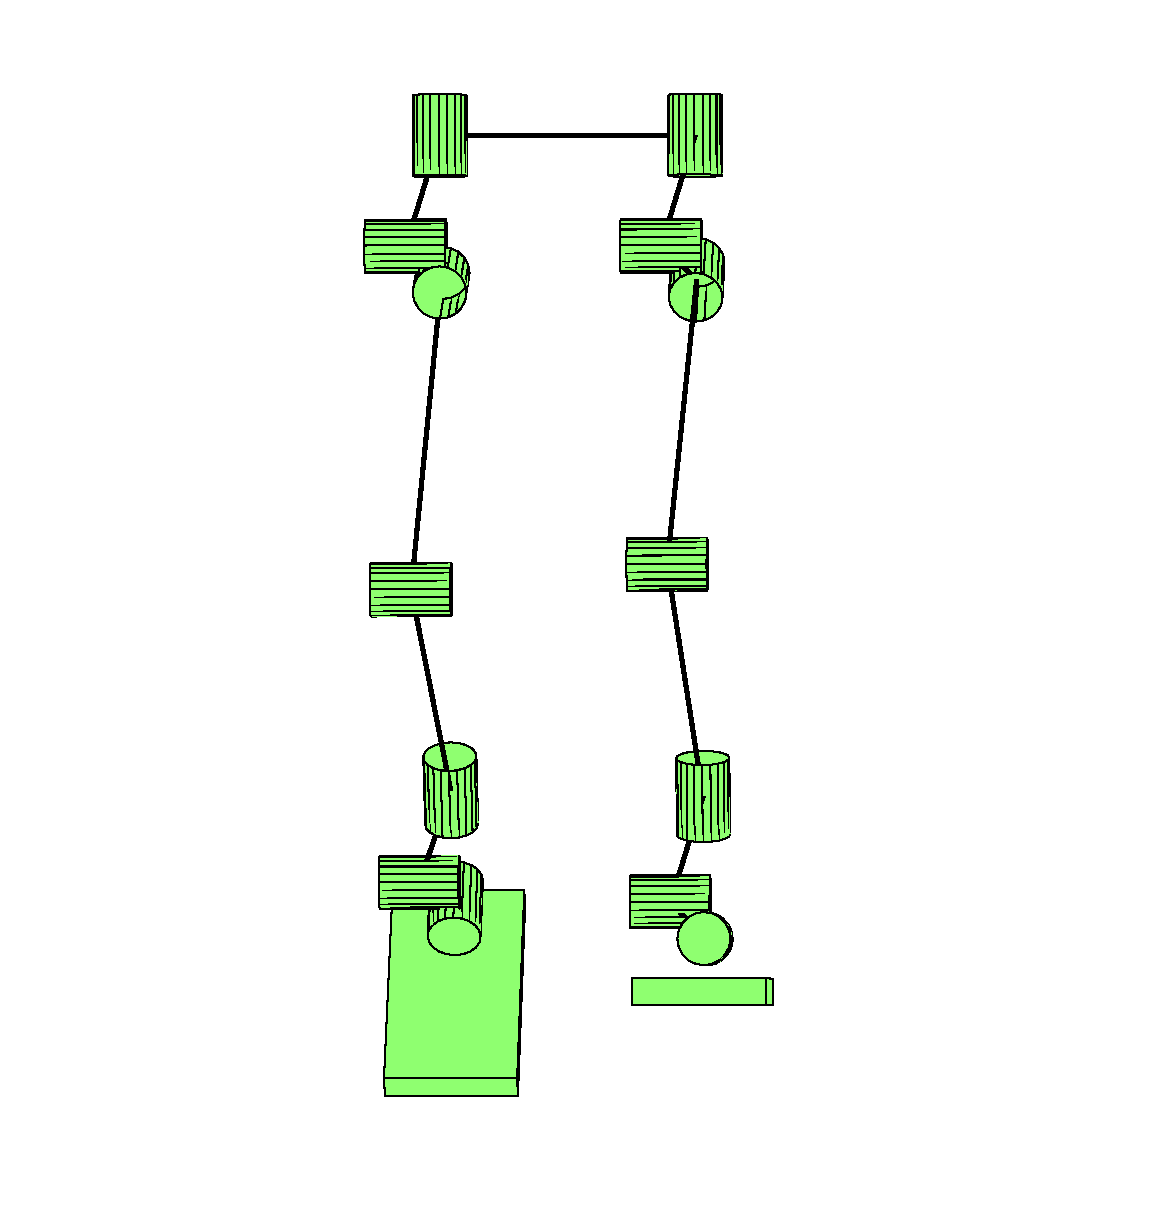
\includegraphics[scale=0.6]{fig/design/ulinkdrawn.eps}
	\end{center}
  \caption{Screenshot of robot structure drawn from the uLINK definition generated directly from CAD.}
  \label{fig:ulinkdrawn}
\end{figure}

With the \texttt{uLINK} structure generated, any of the preprogrammed routines in the toolbox can be used. The toolbox provides a function \texttt{ForwardDynamics} to compute the direct dynamics model using the RNE algorithm. However, the calculations omit the effects of any external forces acting on the system. Since it is important to incorporate the contribution of the ground reaction forces, the toolbox was modified to model the complete dynamics of the system. 

\subsection{Contact Modeling} % (fold)
\label{sub:initial_contact_modeling}

One challenging aspect of dynamic simulations is to accurately model the effects of external forces on the system during the stance phase. To emulate the ground reaction forces during this period of the gait cycle, a contact model is used to generate an approximate contact force. For the initial design specifications, a spring-damper contact model is used (shown in Figure~\ref{fig:springdamper}). Both feet are modelled as point contacts which experience a normal force proportional to the output of the spring-damper system when in contact with the ground. A more complex version of (\ref{eq:contactf}) is used for full dynamic simulations in later chapters (Section~\ref{sub:full_contact_modeling}).

\begin{figure}[!b]
	\begin{center}
    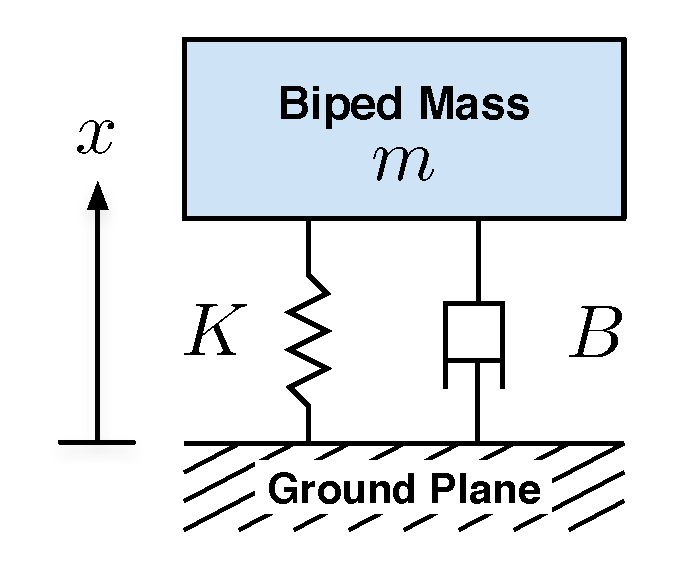
\includegraphics[width=100mm]{fig/design/springdamper.eps}
	\end{center}
  \caption{System diagram of spring-damper contact model used in dynamic simulations.}
  \label{fig:springdamper}
\end{figure}

To incorporate the effects of ground contact into the existing dynamic model, the resulting force produced by (\ref{eq:contactf}) is injected into the RNE algorithm between the end of the first pass and the start of the second pass. At the start of the second pass, the external contact force is used to initialize the backwards recursion. 

\begin{equation}
	\label{eq:contactf}
	F_{normal} = B{\dot{x}} + Kx
\end{equation}

The contact force proportional to the output of the spring-damper system (\ref{eq:contactf}) was used to initialize the backwards pass as shown in Listing~\ref{contactcode}:

\begin{lstlisting}[label=contactcode,caption=Contact force injection in RNE backwards recursion.]
if uLINK(RCONTACT).p(3) < 0.0
	Kr = K;	 % Spring Constant
	Br = B;  % Damper Constant
	
	% Velocity of the Contact Point in World Frame:
	vr = uLINK(RCONTACT).vo + cross(uLINK(RCONTACT).w, uLINK(RCONTACT).p); 
	
	% Normal Force Exerted by Spring-Damper Contact Model:
	N = -Kr*uLINK(RCONTACT).p(3)-Br*vr(3);
	
	% Inject Normal Force Into RNE Backwards Pass Initialization:
	FCR = [0 0 N]';
else
	FCR = [0 0 0]'; 
end
\end{lstlisting}

The variables \texttt{Kr} and \texttt{Br} represent the spring and damper coefficients in the spring-damper contact model. \texttt{RCONTACT} is a constant link number representing the point contact foot. The velocity due to the point foot coming in contact with the ground (\texttt{vr}) is recomputed by considering the original velocity (\texttt{vo}) and the cross product between the position of the foot (\texttt{uLINK.p}) and angular velocity (\texttt{uLINK.w}). The resulting normal force is computed and injected into the backwards pass if the foot position is below the ground level (condition shown in line 1). With this modification included, the complete direct dynamics can be used to obtain the joint torques during an estimated gait cycle for the initial design specification.   
% subsection modifications (end)

% section contact_modeling (end)

% section kajita_s_matlab_toolbox (end)

\subsection{Gait Estimation} % (fold)
\label{sec:gait_estimation}
	
In order to emulate the operating conditions for the 14 DOF bipedal robot, the dynamic simulation must include all dynamic effects experienced during a complete gait cycle. One method of emulating the normal operating conditions is to use human gait as an estimate. While it is ambitious to expect a bipedal robot to match the performance of human-like walking, it provides a basis from which the initial selection of electromechanical components can be made. The goal is to extract the kinematic parameters experienced by the human limbs while walking and impose similar conditions on the robot in dynamic simulation. Given these constraints, the inverse dynamics problem can be solved to obtain the joint torque estimates during various stages of the gait cycle. Coupled with the modifications to emulate contact forces during the stance phase, this approach provides a fast method of estimating the torque loading at each joint to develop the initial design specification. 
	
In order to use kinematic parameters from human gait, data published from the 2008 Dynamic Walking conference was used \cite{dw2008}. The published dataset used sensors to measure the joint angles and velocities of lower body human limbs under several gait cycle speeds (fast, slow and normal walk). This raw sensory data was imported into the Matlab environment using a 3D motion analysis toolbox BodyMech \cite{bodymech}. This information was incorporated into the dynamic simulation by enforcing the joint angles, velocities and accelerations from each captured frame of the reference dataset. The forced joint parameters were assigned to the global \texttt{uLINK} structure to be used in conjunction with the RNE-based inverse dynamics algorithm. 

\begin{figure}[!h]
	\begin{center}
	\begin{tabular}{cc}
	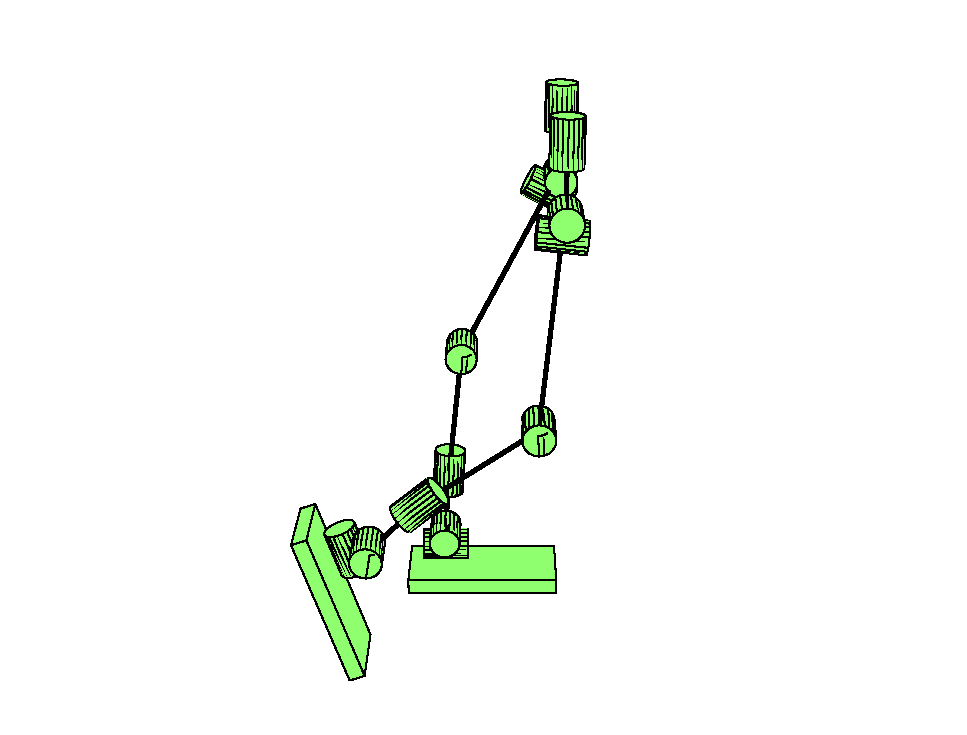
\includegraphics[scale=0.5]{fig/design/ulinkwalk1.eps} &
    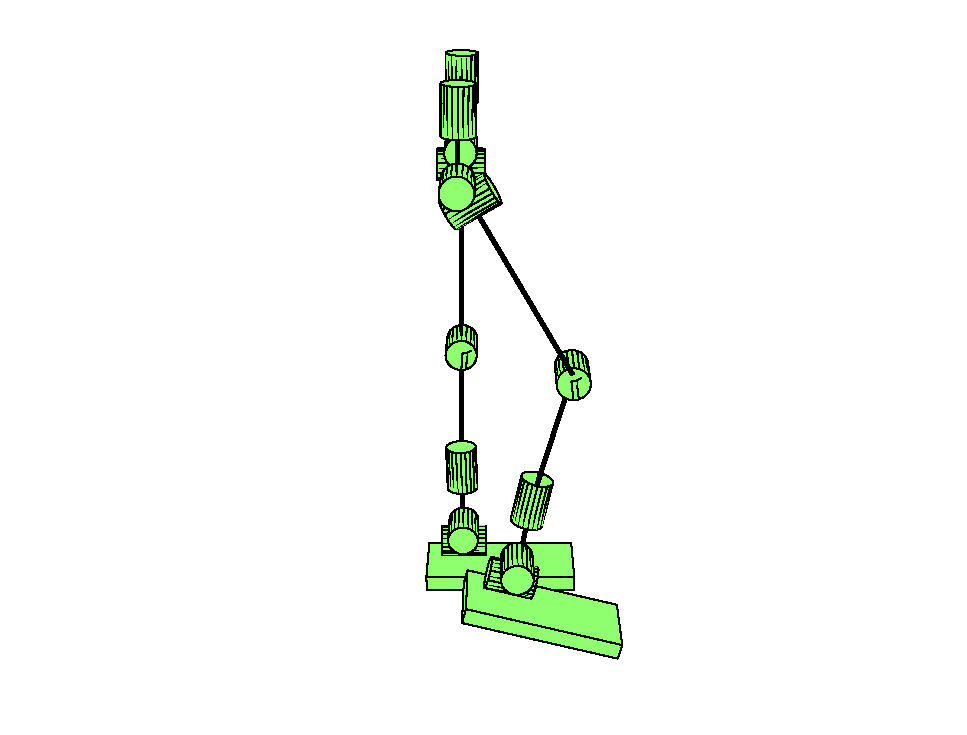
\includegraphics[scale=0.5]{fig/design/ulinkwalk.eps}
	\end{tabular}
	\end{center}
  \caption{Frame captures of the uLINK structure under the estimated gait cycle to obtain initial design specifications.}
  \label{fig:ulinkframes}
\end{figure}

A simulation was implemented in the Matlab environment using a combination of the BodyMech toolbox and Kajita's toolbox. The BodyMech toolbox was used to extract the frame-by-frame 3D kinematic parameters as a human executed the gait cycle. These parameters were processed and stored in order to be played back on the robot model defined by the \texttt{uLINK} structure. To compensate for the differences in size between humans and the small biped, the joint velocities and accelerations were scaled by selecting a different reference gait speed from the published data set. Once the parameters were applied, the RNE-based inverse dynamics algorithm was used to determine the torques at each joint in the structure during the estimated gait. This process was repeated for each frame (illustrated in Figure~\ref{fig:ulinkframes}) in the captured dataset and the results of robot's kinematics/dynamics ($\q$, $\vec{\dot{q}}$, $\vec{\ddot{q}}$ and $\vtau$) were tabulated for post processing. 
% section gait_estimation (end)


\subsection{Initial Design Specifications} % (fold)
\label{sec:initial_design_requirements}
The results of the dynamic simulations under human-gait analysis form the basis for the initial electromechanical components selection process. As expected, it was observed that the largest demands in torque loading on each of the joints occurred during the stance phase immediately after the heel strike. The torque demands at that instant spike immediately to almost three times the steady state torque loading on the joints. 

% \begin{figure}[!h]
% 	\begin{center}
%     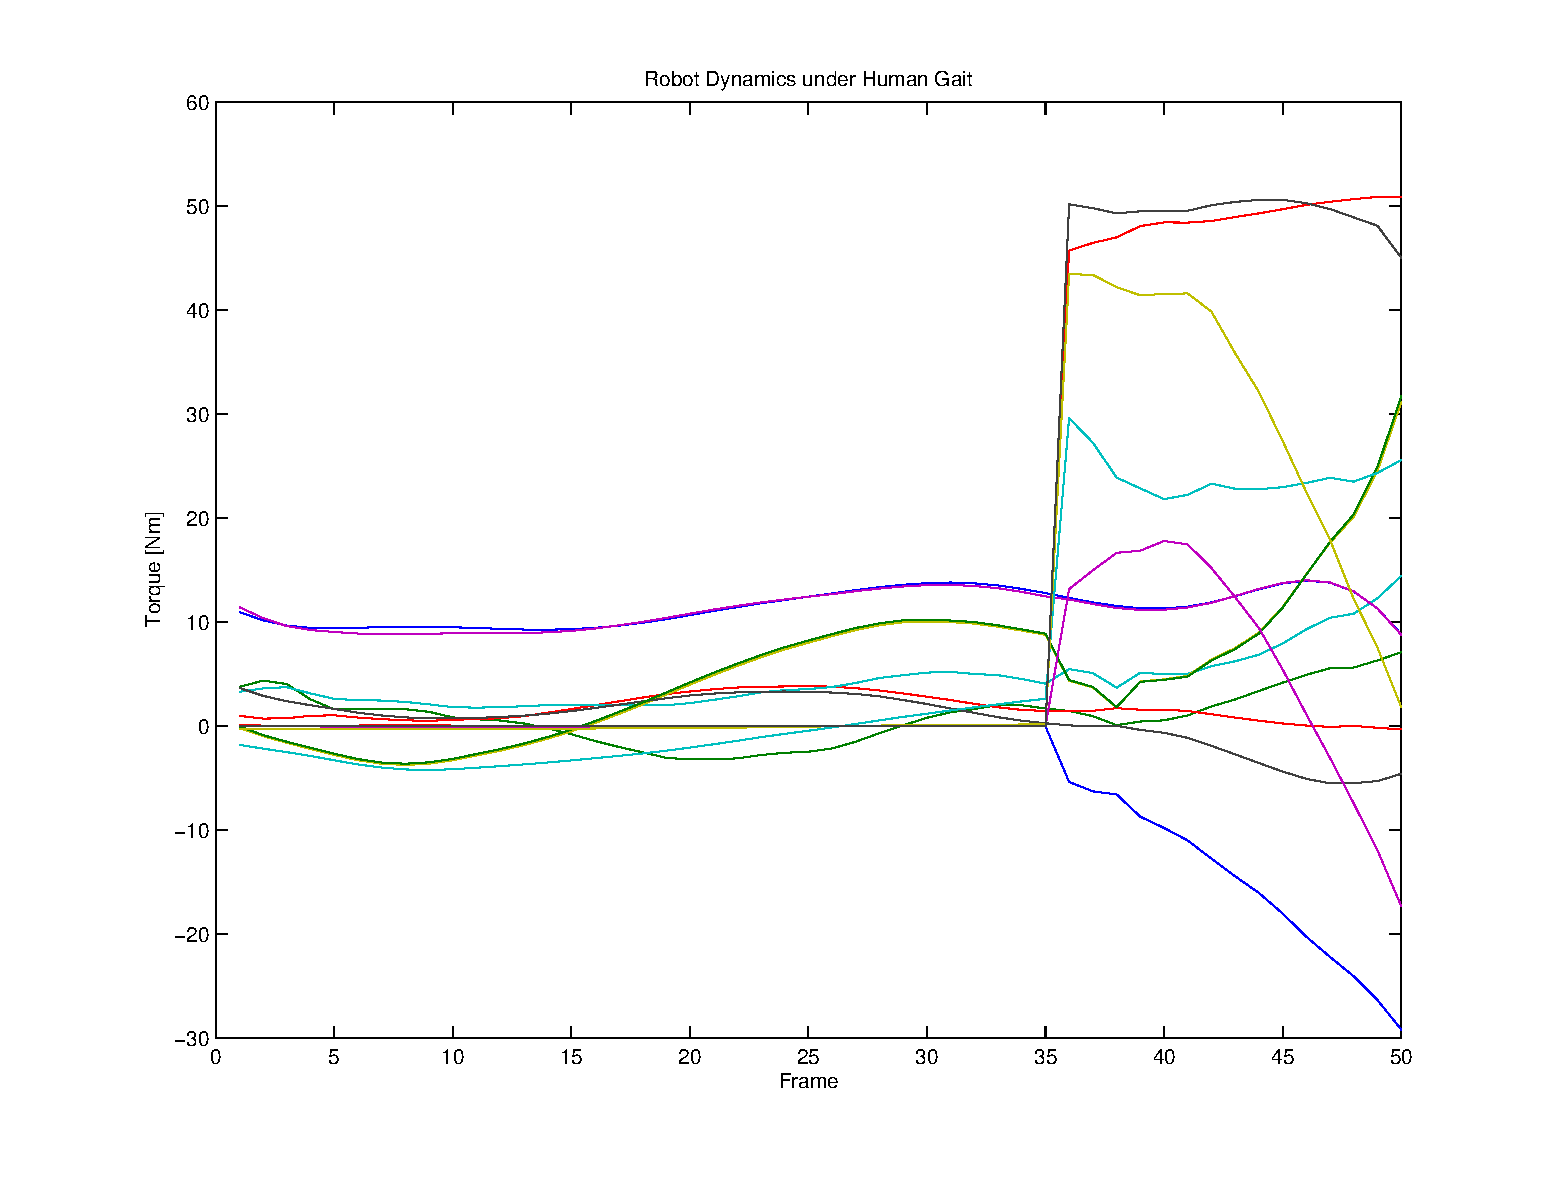
\includegraphics[scale=0.6]{fig/design/gaitplot.eps}
% 	\end{center}
%   \caption{Joint torque profile during the estimated gait cycle obtained from a published data set.}
%   	\label{fig:gaitplot}
% \end{figure}

Selecting motor specifications based only on the peak torque requirements would result in large and overpowered actuators for the continuous operational loads. The secondary design objective is to keep the overall system mass low, making it desirable to minimize the actuator size since it contributes to the majority of the weight in the system. 

Motor manufacturers specify rated conditions for \emph{continuous} operation, while the peak torque demands in this application only exist for a short period of time when ground contact is made. It is possible to safely push DC motors beyond the nominal rated capacities for short periods of time by considering the maximum mechanical power output and thermal characteristics. Therefore, it is desirable to select motors primarily on the steady state torque load requirements while investigating other characteristics to ensure that they can handle the peak load requirements. 

\begin{table}[!h]
  \centering
  \caption{Individual joint torque demands for each DOF in one leg using gait estimation.}
    \begin{tabular}{lcc}
    \addlinespace
    \toprule
    \textbf{Joint} & \textbf{Normal} & \textbf{Peak}\\
    \midrule
    Hip Yaw		&	3.698 Nm	&	3.698 Nm\\
    Hip Roll	&	13.606 Nm	&	14.054 Nm\\
    Hip Pitch	&	10.081 Nm	&	38.295 Nm\\
    Knee Pitch  &	5.229 Nm	&	16.539 Nm\\
    Ankle Yaw	&	3.858 Nm	&	3.858 Nm\\
    Ankle Pitch	&	4.395 Nm	&	7.923 Nm\\
    Ankle Roll	&	2.824 Nm	&	5.021 Nm\\
    \bottomrule
    \end{tabular}%
  \label{jointtable}%
\end{table}%

While the torque demands vary for each joint (see Table \ref{jointtable}), the results from the analysis are concatenated to obtain a single set of design specifications. This reduces the number of different models selected from the manufacturer and it also simplifies the electromechanical design process. For the initial design, the normal torque specification is obtained by taking an average of joint torque values during the swing phase. Since the ground reaction forces experienced during the stance phase produce large torques in a short period of time, the peak torque specification is obtained by selecting the highest torque value from all frames. The combined initial design specifications for the drivetrain components are summarized in Table \ref{tab:spectable}.

\begin{table}[!h]
  \centering
  \caption{Initial design specifications for drivetrain components.}
    \begin{tabular}{lcc}
    \addlinespace
    \toprule
    \textbf{Condition} & \textbf{Torque} & \textbf{Velocity}\\
    \midrule
    Normal & 14 Nm & 2.48 rad/s\\
    Peak  & 50 Nm & 6.82 rad/s \\
    \bottomrule
    \end{tabular}%
  \label{tab:spectable}%
\end{table}%

The contact model parameters (spring and damping coefficients) were observed to have a noticeable effect on the peak design specifications. Since the contact model only provides a crude approximation of the ground reaction forces that the real robot will experience, the final selected value was chosen to provide a peak torque which averages between the largest and smallest values. The final hand-tuned spring and damping coefficients used in deriving the design specifications were $K = 10000$ and $B = 100$, respectively. These contact model parameters result in a steady-state ground penetration depth of $0.25cm$. The foot characteristics can be modified to match this behaviour by adding a rubber sole. 
% section chassis (end)

%======================================================================
%   D R I V E T R A I N  S E L E C T I O N
%======================================================================


\section{Drivetrain Selection} % (fold)
\label{sec:drivetrain}
The drivetrain selection process includes selecting the appropriate components to transmit the required torque (as per the initial design specifications) to each joint. The electric machines used to generate mechanical power for the purposes of this project are coreless DC motors. The motors used for the 14 DOF bipedal robot were supplied by Micromo Solutions (part of the Faulhaber Group) \cite{sw:micromo}. The online product catalogue was used as a reference tool for the drivetrain selection process. The majority of the weight contribution of the complete system is attributed to the motors. Therefore, the design objective was to select a combination of motors and appropriately sized gearheads to meet the design specifications while keeping the overall mass of the system as low as possible. The remainder of this section presents the selection of appropriate motor and gearhead combinations to meet the design objectives. 

\subsection{Mechanical Power Requirements} % (fold)
\label{sub:mechanical_power_requirements}
To narrow down the selection process into a subset of the motors which meet the initial design specifications, preliminary mechanical power calculations are performed. The mechanical power output required by each generator is specified by the required torque ($\tau$) and speed ($\omega$) of the motor: 

\begin{equation}
	P = \tau \times \omega
\end{equation}

The initial specifications for the drivetrain components listed in Table \ref{tab:spectable} list two values for the torque. As mentioned previously, designing the system to meet the peak torque requirements would yield significantly larger motors and increase the overall mass. Instead, it is desirable to design the system to meet the average (continuous) torque requirements and ensure that the system is capable of withstanding the large impulsive forces experienced at the impact points of the gait cycle. Therefore, the initial mechanical power requirement calculation is based on the normal or average torque loading on the joints (14Nm). While no speed requirements were specified in the initial design specifications, the tabulated kinematic and dynamic data collected from the dynamic simulation was used to compute the average speed experienced by the joints and the largest value was selected for the purposes of calculation. This provides an additional buffer in the mechanical power considerations since not all joints are likely to experience the highest speed. The average speed calculated from the dynamic simulation was found to be 65RPM. Substituting these values along with the conversion factor for units: 

\begin{equation}
	P = \tau \times \omega = 14Nm \times 65RPM \times 0.1047 = 95.28W
\end{equation}

Note that due to the assumptions made in calculating this value, 95.28W represents an upper bound on the amount of power the design should be capable of providing. Therefore the potential solution candidates should be rated for the nominal power around the region of this value. The analysis tools presented in the following sections were used to evaluate the remaining actuation solution candidates. 

First, DC motors were analyzed based on their torque-speed (Section~\ref{sub:torque_speed_analysis}), power and efficiency (Section~\ref{sub:power_and_efficiency_analysis}) and thermal (Section~\ref{sub:thermal_analysis}) characteristics. Full DC motor plots are shown for the final selection since the selection of gear ratio was treated as a separate design decision. With the appropriate motor selected, compatible gearhead solutions were analyzed to select the reduction ratio which met the design specifications (Section~\ref{sub:final_configurations}). 
% subsection mechanical_power_requirements (end)

\subsection{Torque-Speed Analysis} % (fold)
\label{sub:torque_speed_analysis}
The primary tool used to analyze and compare alternative solutions is the torque-speed graph. Analysis of this graph is used to address the peak requirements. Given the structure of the motor specifications provided by Micromo Solutions, a spreadsheet was constructed to automatically generate the torque-speed characteristics from the motor constants. These constants were pre-populated from the manufacturer specification sheets and the torque-speed graphs were automatically generated. 

\begin{equation}
	\omega = \omega_{no-load} - k\tau
\end{equation}

The relationship between the torque of the motor and the speed of the revolving shaft is approximately linear so it is typically specified by a slope constant for the curve. While the constant $k$ is usually provided as a positive value, the slope of the torque-speed curve is negative (i.e. as the torque increases the speed decreases). The full torque-speed profile of the final motor selection is shown in Figure~\ref{fig:torquespeed}. 

\begin{figure}[!t]
	\begin{center}
    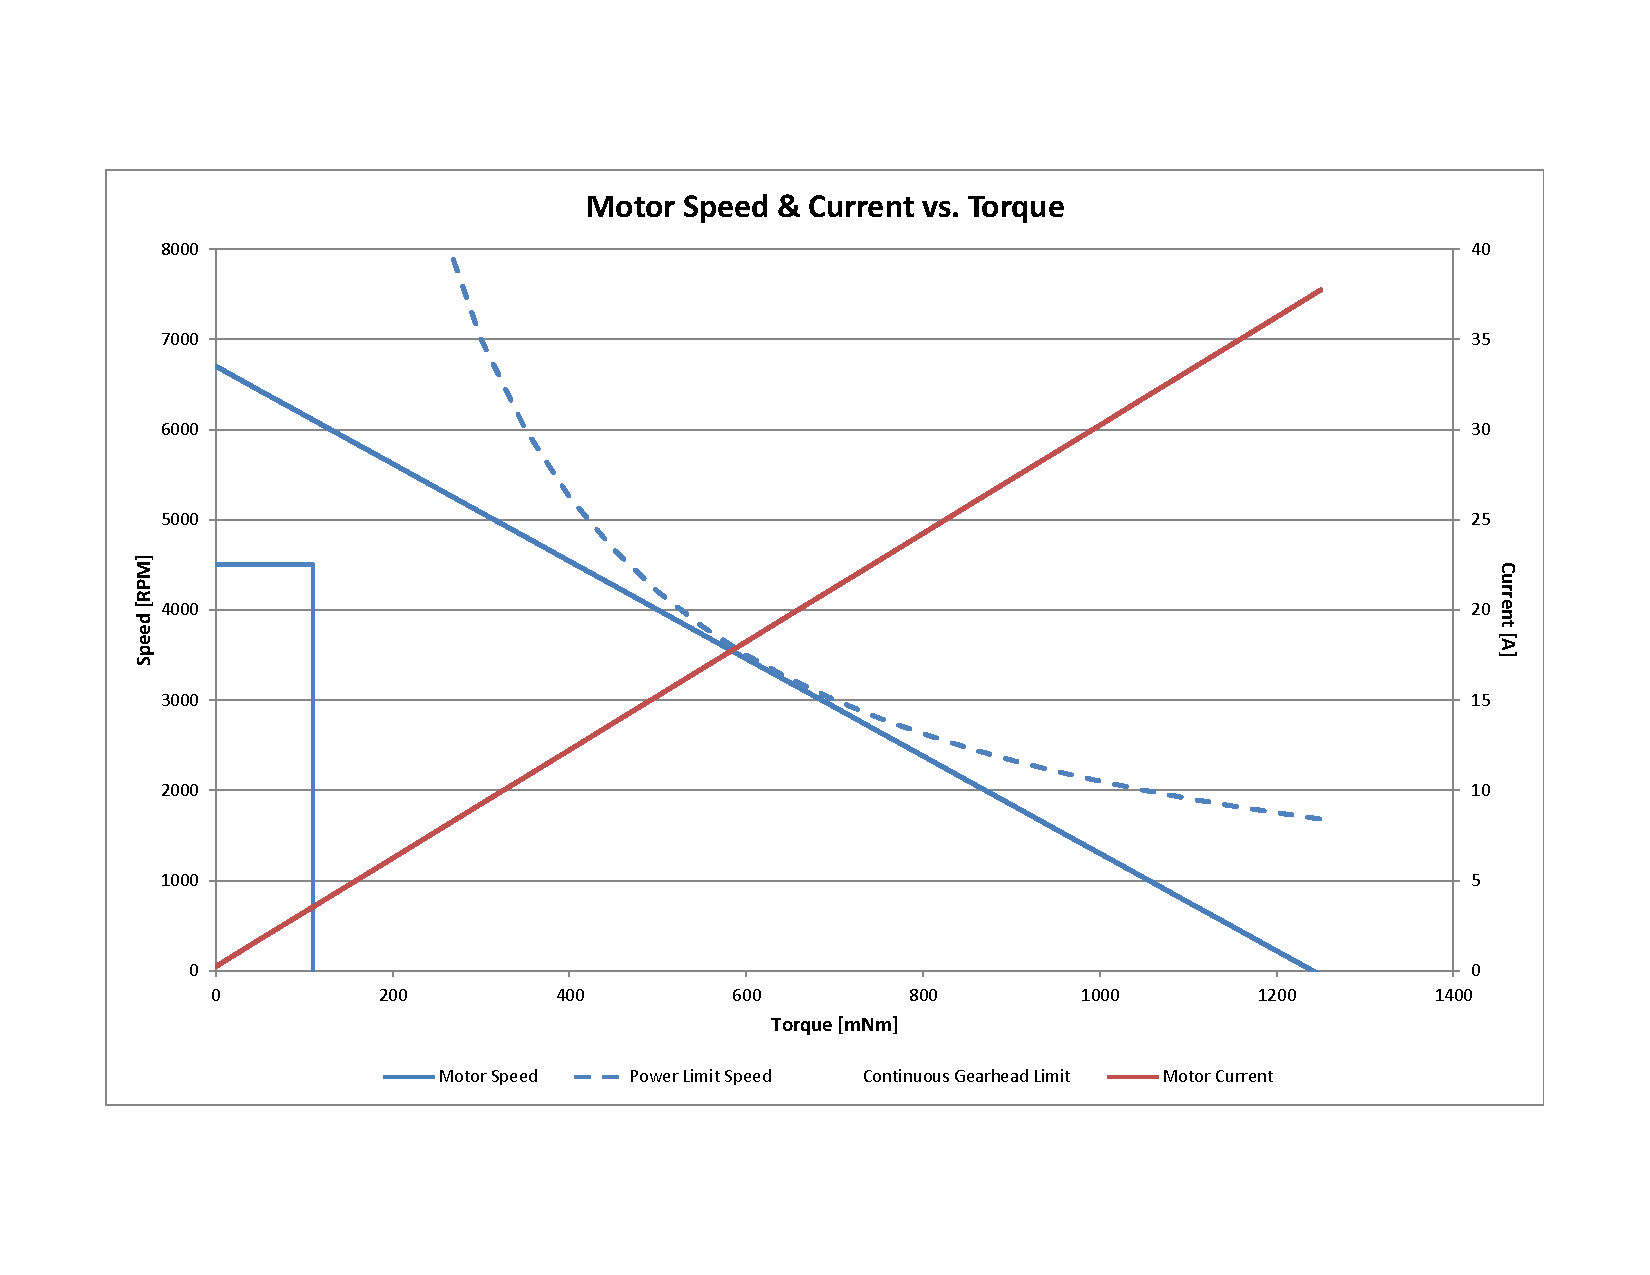
\includegraphics[trim = 20mm 30mm 20mm 30mm,clip,width=15cm]{fig/design/motor1.pdf}
	\end{center}
  \caption{Micromo 3257CR Coreless DC Motor: Speed and Current vs Torque}
  \label{fig:torquespeed}
\end{figure}

% subsection torque_speed_analysis (end)

\subsection{Power and Efficiency Analysis} % (fold)
\label{sub:power_and_efficiency_analysis}
Another key factor in comparing drivetrain components is the relationship between the power produced and the overall efficiency of the motor as a function of its torque. The efficiency curve compares the ratio of electrical power input to mechanical power output. While it is typically desirable to operate the motor at its peak efficiency, the torque demands fluctuate throughout the gait cycle making it difficult to base the motor selection process on this basis alone. However, it is desirable to ensure that the motor is reasonably efficient around the bounds of operation. The power and efficiency profile of the final motor selection is shown in Figure~\ref{fig:powerefficiency}. 

\begin{figure}[!t]
	\begin{center}
    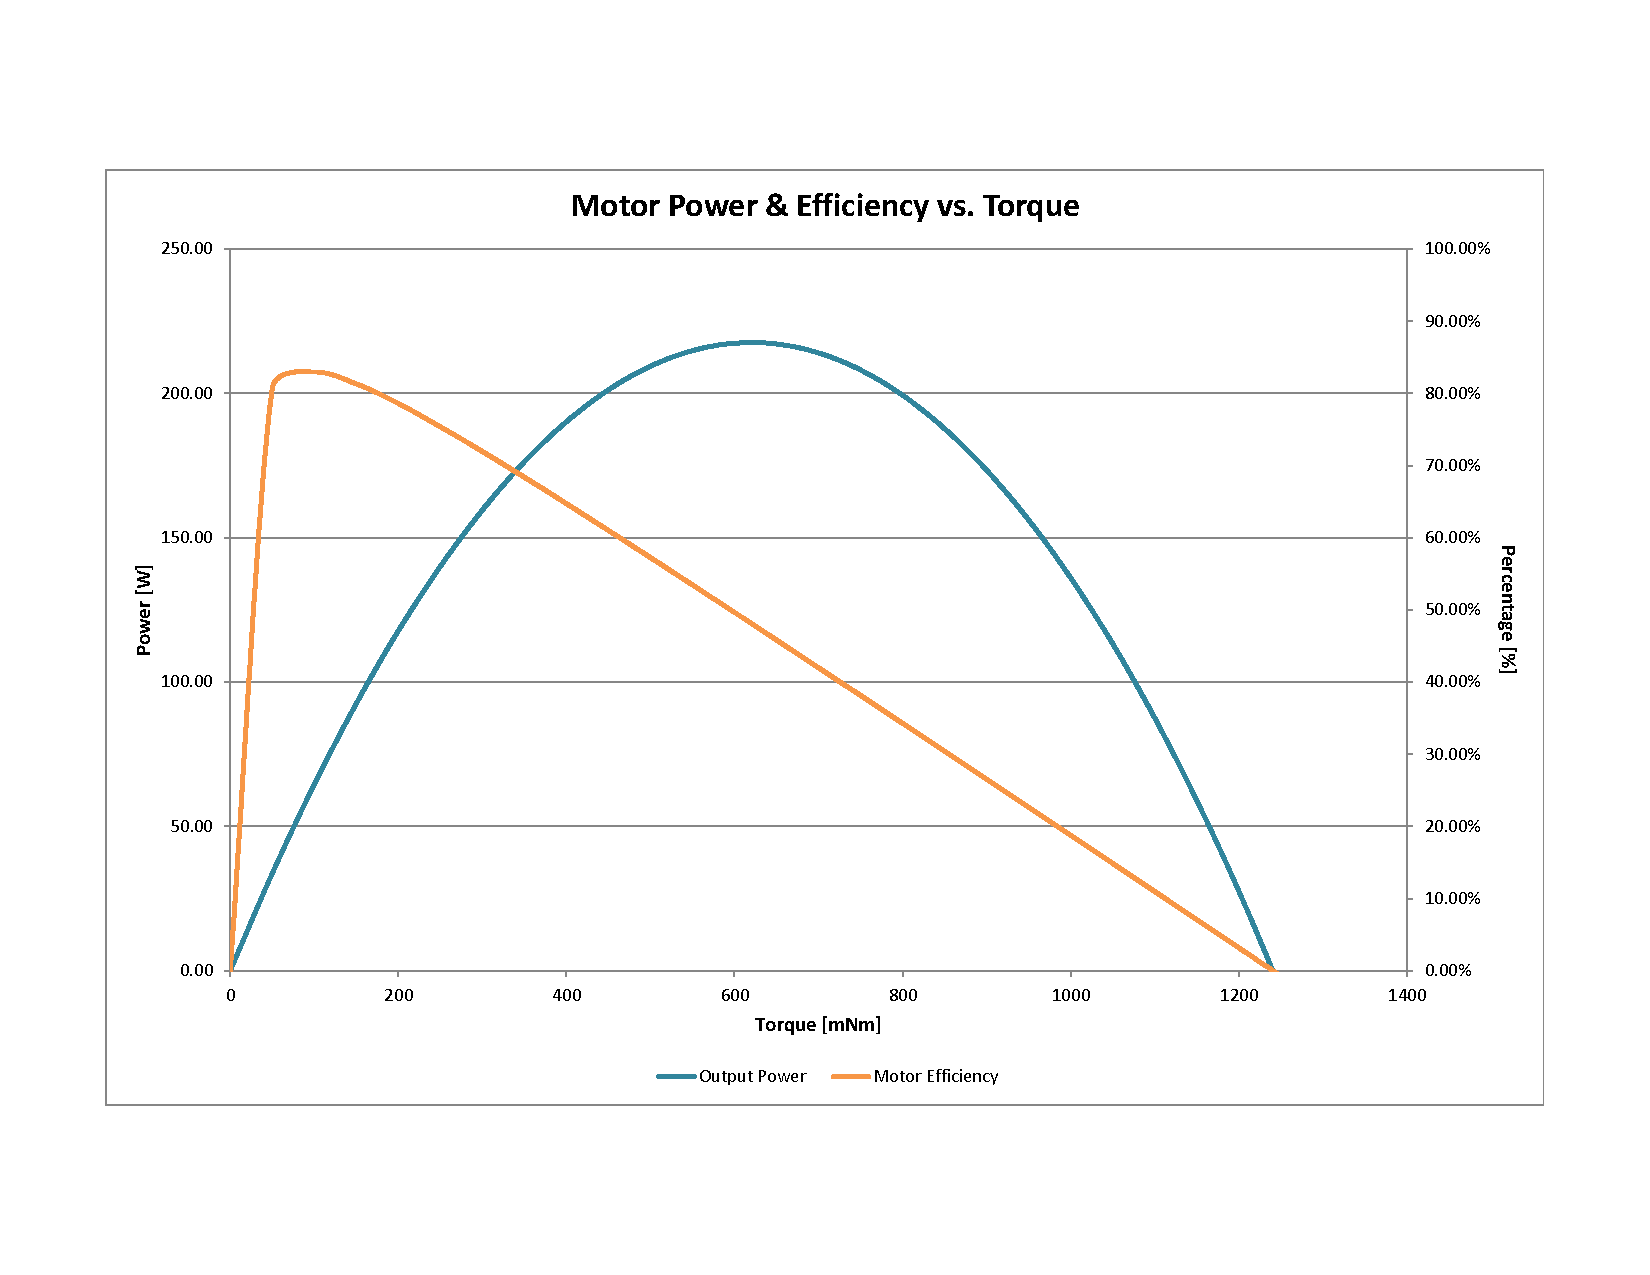
\includegraphics[trim = 20mm 30mm 20mm 30mm,clip,width=15cm]{fig/design/motor2.pdf}
	\end{center}
  \caption{Micromo 3257CR Coreless DC Motor: Power and Efficiency vs Torque}
  \label{fig:powerefficiency}
\end{figure}

% subsection power_and_efficiency_analysis (end)

\subsection{Thermal Analysis} % (fold)
\label{sub:thermal_analysis}
As mentioned previously, out of the initial design specifications the motor selection process is based on the continuous or average torque loading on the joints. However, during each gait cycle the torque demands peak due to external, impulsive force interaction with the environment (i.e. heel-strike). While these peaks may be outside of the motor's continuous operating range for a very short period of time, the heat generated inside the motor core can build up and cause significant damage. Another consideration is the effect of thermal build up of the motor under continuous use at the specification of 14Nm. Therefore it is necessary to generate thermal plots alongside the torque-speed analysis to verify that the selected motors can withstand the temperature rise during operation. Given an assumed value for the ambient temperature, the total temperature of the motor can be calculated as: 

\begin{equation}
	T_{total} = T_{ambient} + T_{inc}
\end{equation}

Where the temperature increase inside the motor core is provided by the following relationship\footnote{The thermal characteristic equations were obtained from the manufacturer's technical documents on motor calculations available at \url{http://www.micromo.com/motor-calculations.aspx}}: 

\begin{equation}
	T_{inc} = I^{2}R \times (R_{th1} + R_{th2})
\end{equation}

$I$ and $R$ are the current through and the resistance of the motor windings, respectively. Constants $R_{th1}$ and $R_{th2}$ are specified by the motor manufacturer. The thermal characteristics of the final motor selection is shown in Figure~\ref{fig:thermal}.


\begin{figure}[!t]
	\begin{center}
    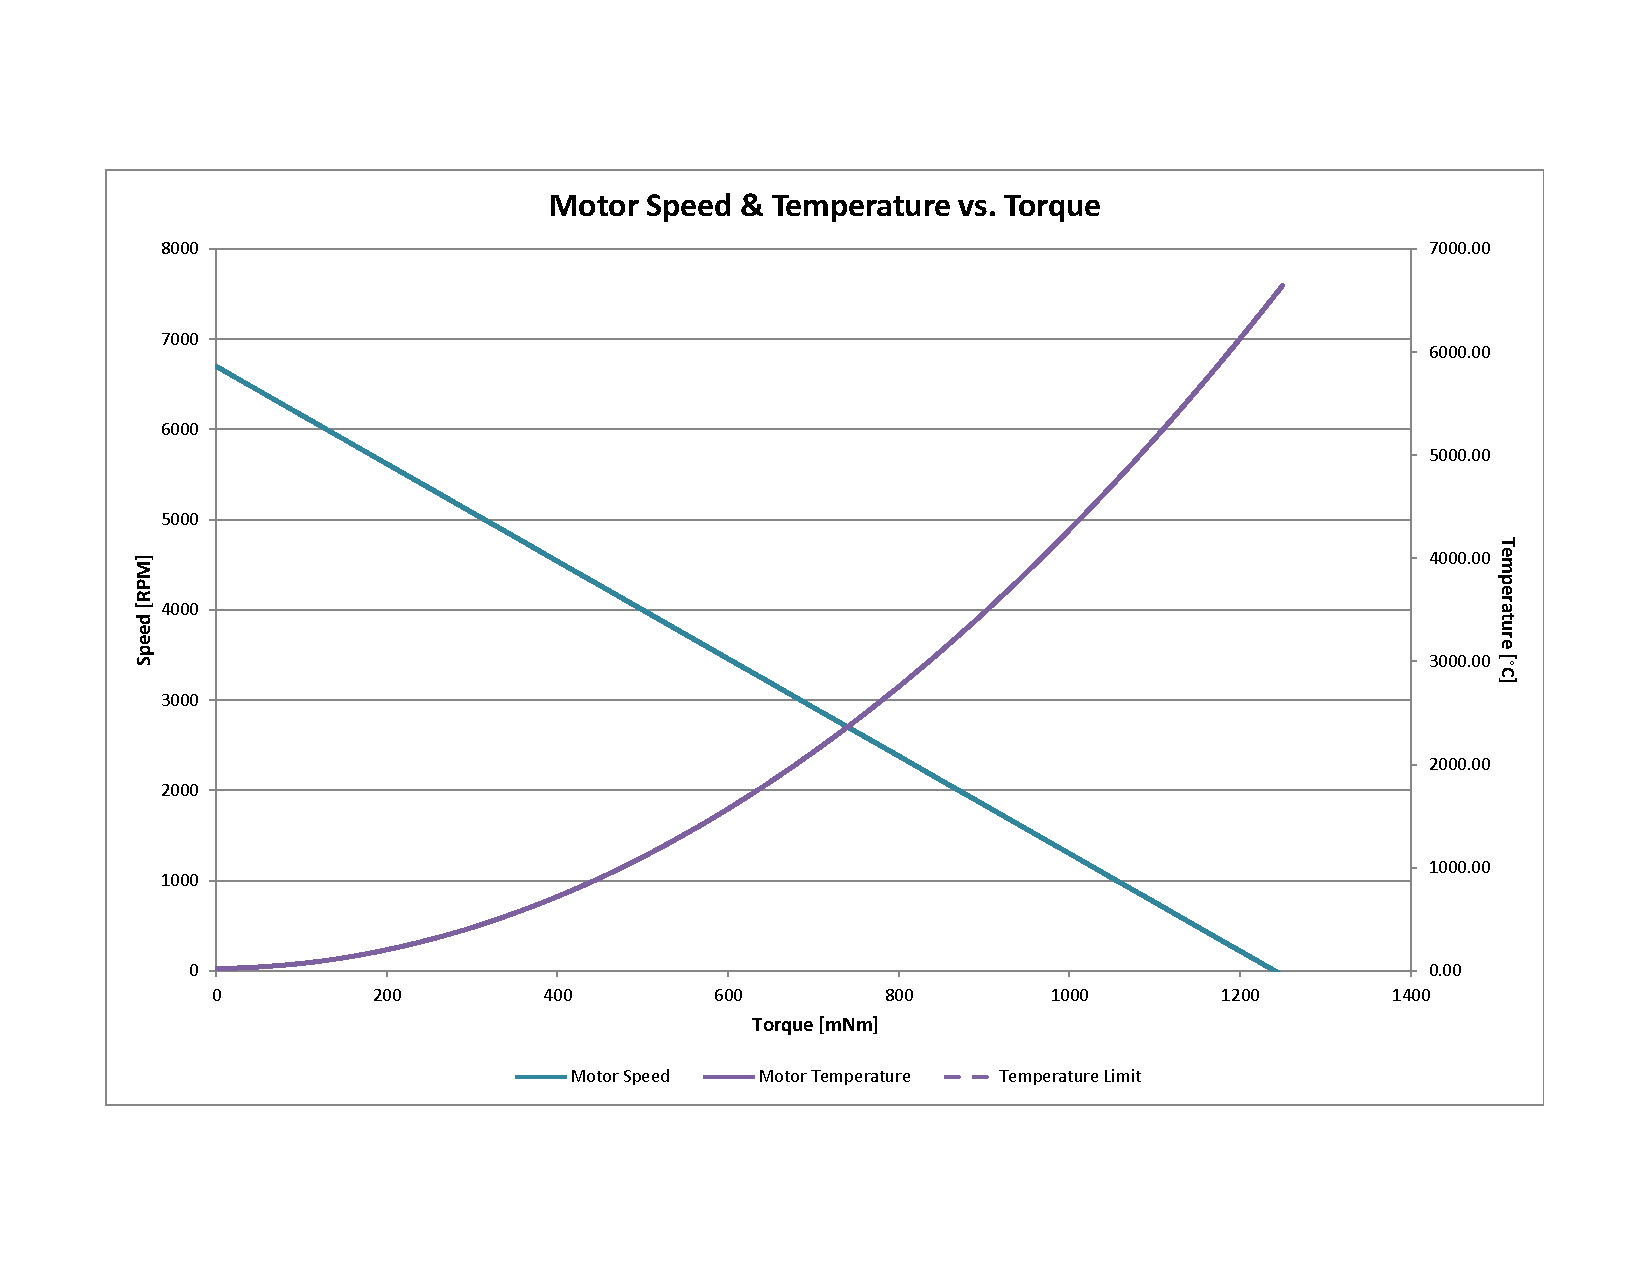
\includegraphics[trim = 20mm 30mm 20mm 30mm,clip,width=15cm]{fig/design/motor3.pdf}
	\end{center}
  \caption{Micromo 3257CR Coreless DC Motor: Speed and Temperature vs Torque}
  \label{fig:thermal}
\end{figure}
% subsection thermal_analysis (end)

\subsection{Final Configurations} % (fold)
\label{sub:final_configurations}
Aside from the torque-speed, power, efficiency and thermal analyses, there are several other considerations which factor into the design  while selecting drivetrain components. These considerations pertain to the secondary objective to minimize the overall weight of the system while simultaneously shifting the COM higher. Between the motor and the gearhead, the majority of the weight comes from the actual coreless DC motor so it is desirable to select a smaller (lighter) motor and meet the specified torque requirements by increasing the gear reduction ratio. Another consideration is the physical size of the motor itself, as the diameter and length of each motor vary significantly between different offerings. Since gearheads are coupled directly onto the motor shaft, the complete drivetrain assembly is usually long. 

\begin{figure}[!t]
	\begin{center}
    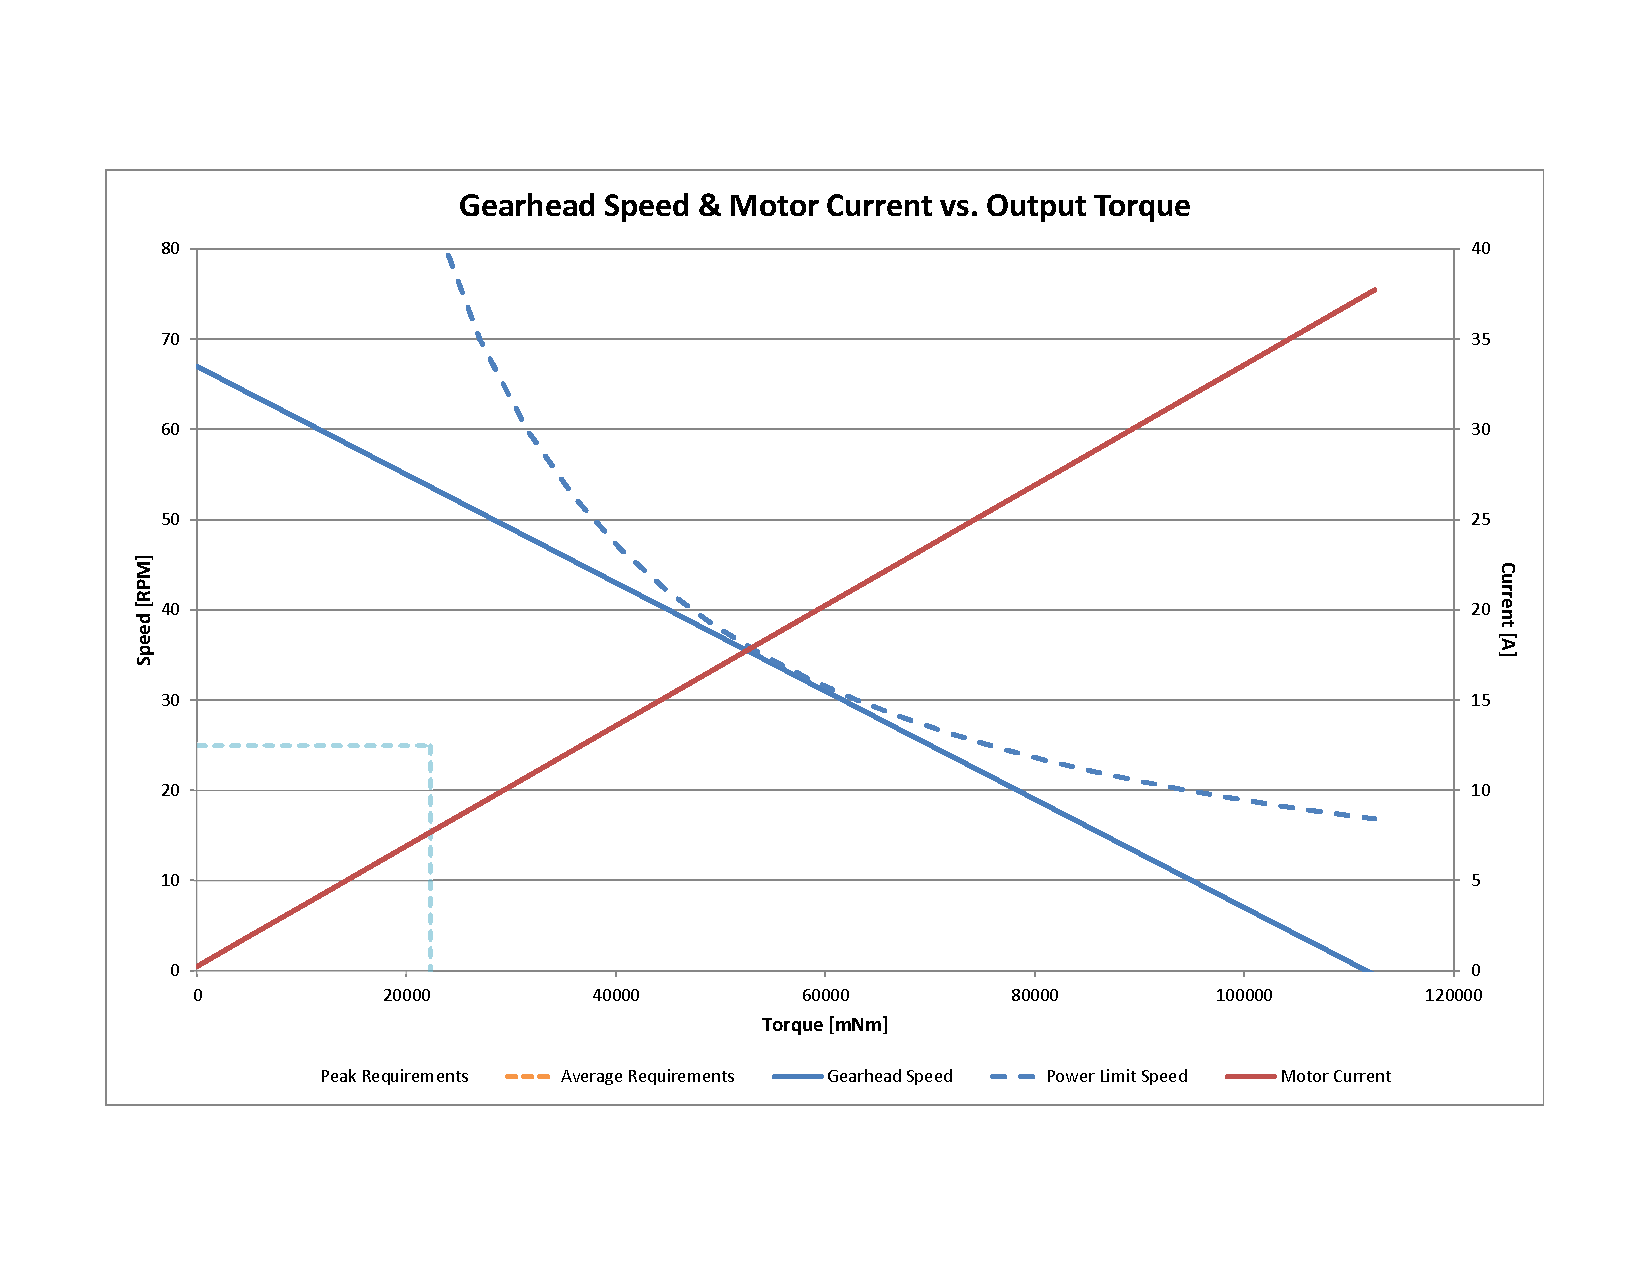
\includegraphics[trim = 33mm 25mm 20mm 25mm,clip,width=15cm]{fig/design/gearhead1.pdf}
	\end{center}
  \caption{Micromo 38A Precision Gearhead: Speed and Current vs Torque}
  \label{fig:micromo38a}
\end{figure}

Given these considerations and the analysis in the previous sections, a coreless DC motor from the Micromo Solutions catalog was selected  (Model \#: 3257CR). This motor achieved all of the primary design considerations (average torque requirements, operating within a stable thermal region). Coupled with the motor is a precision gearhead which is capable of producing torques slightly above the initial design specification requirements. The torque-speed characteristics at the gearhead shaft (as shown in Figure~\ref{fig:micromo38a}) are used to verify that the mechanical power output meets the design specification for normal operation. 

While it is desirable to limit the number of different motor and gearhead combinations, it was determined that this combination of drivetrain components was vastly overpowered for the very last joint on the leg (ankle roll). A second combination of motor and gearhead was selected specifically for this joint to reduce the overall mass and raise the COM while meeting the lower joint requirements. This approach improves the controllability of the final system while limiting the total number of different design configurations. The final higher and lower power configurations are defined in Tables \ref{tab:higherconfig} and \ref{tab:lowerconfig}, respectively. 

\begin{table}[!h]
  \centering
  \caption{Higher configuration of motor and gearhead combination from Micromo.}
    \begin{tabular}{lcccc}
    \addlinespace
    \toprule
    \textbf{Model} & \textbf{Mass} & \textbf{Length} & \textbf{Stall Torque} & \textbf{Max Power}\\
    \midrule
    3257CR 12V Motor	&	242g	&	57mm	&	0.547Nm		&	84.50W	\\
    38A 240:1 Gearhead	&	410g	&	80mm	&	20.0Nm		&	-	\\
    \bottomrule
    \end{tabular}%
  \label{tab:higherconfig}%
\end{table}%

\begin{table}[!h]
  \centering
  \caption{Lower configuration of motor and gearhead combination from Micromo.}
    \begin{tabular}{lcccc}
    \addlinespace
    \toprule
    \textbf{Model} & \textbf{Mass} & \textbf{Length} & \textbf{Stall Torque} & \textbf{Max Power}\\
    \midrule
    3242CR 12V Motor	&	172g	&	42mm	&	0.193Nm		&	27.30W	\\
    32A 68:1 Gearhead	&	240g	&	57mm	&	6.0Nm		&	-	\\
    \bottomrule
    \end{tabular}%
  \label{tab:lowerconfig}%
\end{table}%
% subsection final_configurations (end)
% section drivetrain (end)

\section{Mechanical Design} % (fold)
\label{sec:chassis}

The mechanical design of the 14 DOF bipedal robot starts from the initial motor selection presented in the previous section. The 3D CAD models for each motor and gearhead combination are obtained directly from the manufacturer. The design goals for the mechanical chassis are to produce a solid light weight structure which is capable of withstanding external forces from the environment during gait and the applied torques from each joint. The secondary design objective of minimizing the overall weight while shifting the COM higher must also be addressed through the mechanical design. 

\subsection{Anthropometric Dimensioning} % (fold)
\label{sub:anthropometric_dimensioning}
The goal for the 14 DOF bipedal robot is to achieve walking with human-like gait. To this end, anthropometric dimensioning is used as a starting point for the mechanical chassis design. Starting from a soft height requirement of the full lower body, the relative lengths are obtained for the main linkages (i.e. thigh, shank) from the anthropometric resource shown in Figure~\ref{fig:anthropo}. 

\begin{figure}[!h]
	\begin{center}
    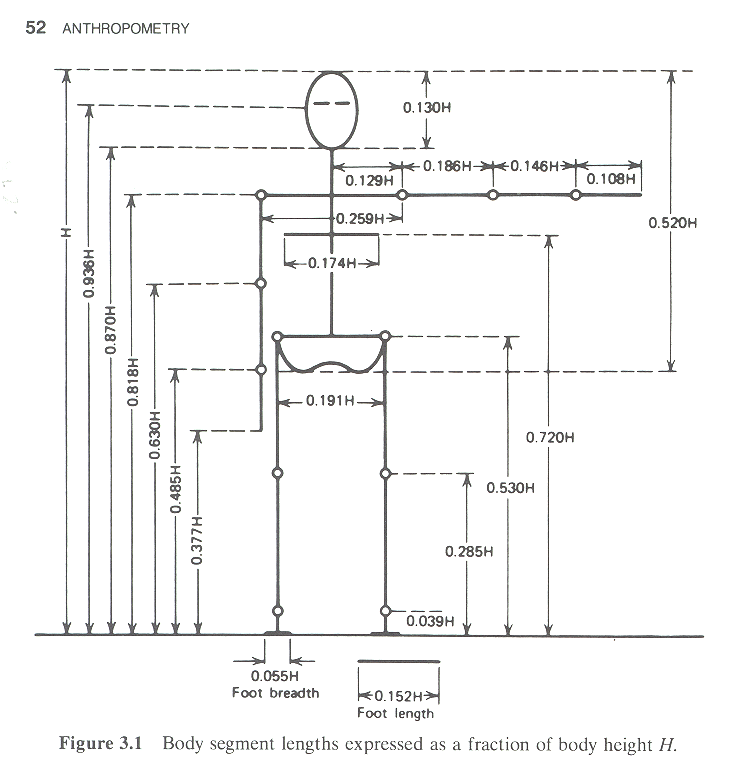
\includegraphics[width=100mm]{fig/design/anthropo.png}
	\end{center}
  \caption{Resource for anthropometric dimensioning of lower body segments \cite{wintergait}.}
\label{fig:anthropo}
\end{figure}
	
Given the ratios between major body segment lengths, a rough estimate for each of the chassis segment lengths is derived and summarized in Table \ref{tab:anthropo}. Note that these dimensions were only used as a starting point. The overall length of the drivetrain components (i.e. motor and gearhead combination) is an additional constraint which can limit how close the final chassis design is to the estimated segment lengths.  

\begin{table}[!h]
  \centering
  \caption{Estimated segment lengths based on anthropometric dimensioning}
  \label{tab:anthropo}%
    \begin{tabular}{lc}
    \addlinespace
    \toprule
    \textbf{Segment} & \textbf{Height [mm]} \\
    \midrule
    Hip   & 11.32 \\
    Thigh & 277.34 \\
    Shank & 278.47 \\
    Foot  & 44.15 \\
    \bottomrule
    \end{tabular}%
\end{table}

% subsection anthropometric_dimensioning (end)

\subsection{Chassis Structural Design} % (fold)
\label{sub:structural_design}
Aluminum was selected as the light weight rigid material to compose the mechanical chassis, based on the widespread availability of various forms of aluminum stock (i.e. channels, beams, etc) and its (relatively) light weight compared to other metal alloys. More specifically, Aluminum 5052 was selected due to its high fatigue strength. This alloy is also easy to work with for manual machining or computer numerical control (CNC) machine tools. 

The chassis is designed as a light weight but rigid frame to house the drivetrain components (actuators, gears, etc). The amount of stock material used in the frame itself also impacts the overall weight and structural rigidity. For example, a link segment designed from a C-Channel beam is structurally sound (since it is a single solid piece of metal). However, it may be significantly heavier than a link segment composed of multiple pieces. The trade off between minimizing the overall weight and structural rigidity can sometimes be mitigated by using a cross brace between adjacent parallel pieces of a frame.  

The low density of aluminum also helps address the secondary design objective of reducing the overall weight. However, the primary weight contribution to the overall system comes from the drivetrain components. This limits the flexibility for weight manipulation from a purely chassis design standpoint. However, mechanical design techniques can be used manipulate the COM location by strategically positioning the mounting points for motors and gearheads. 
% subsubsection structural_design (end)

\subsection{Mechanical Power Transmission} % (fold)
\label{sub:mechanical_power_transmission}
The biped consists entirely of rotating mechanical joints between link segments. Machine components such as shafts and bearings are used to transmit the rotational mechanical power between links. This type of mechanical coupling is also used to address the secondary objective of shifting the COM position higher. By using components such as miter gears, the mechanical power transmission is be shifted with a perpendicular offset (90$^\circ$). This technique is used to strategically decouple the mounting position of a drivetrain assembly (i.e. motor with fixed gearhead) from the actual axis of rotation. Consequently, this decoupling is used to relocate motors such that the weight distribution is manipulated in favour of having a higher COM position (illustrated in Figure \ref{fig:miter}).
	
\begin{figure}[!h]
	\begin{center}
    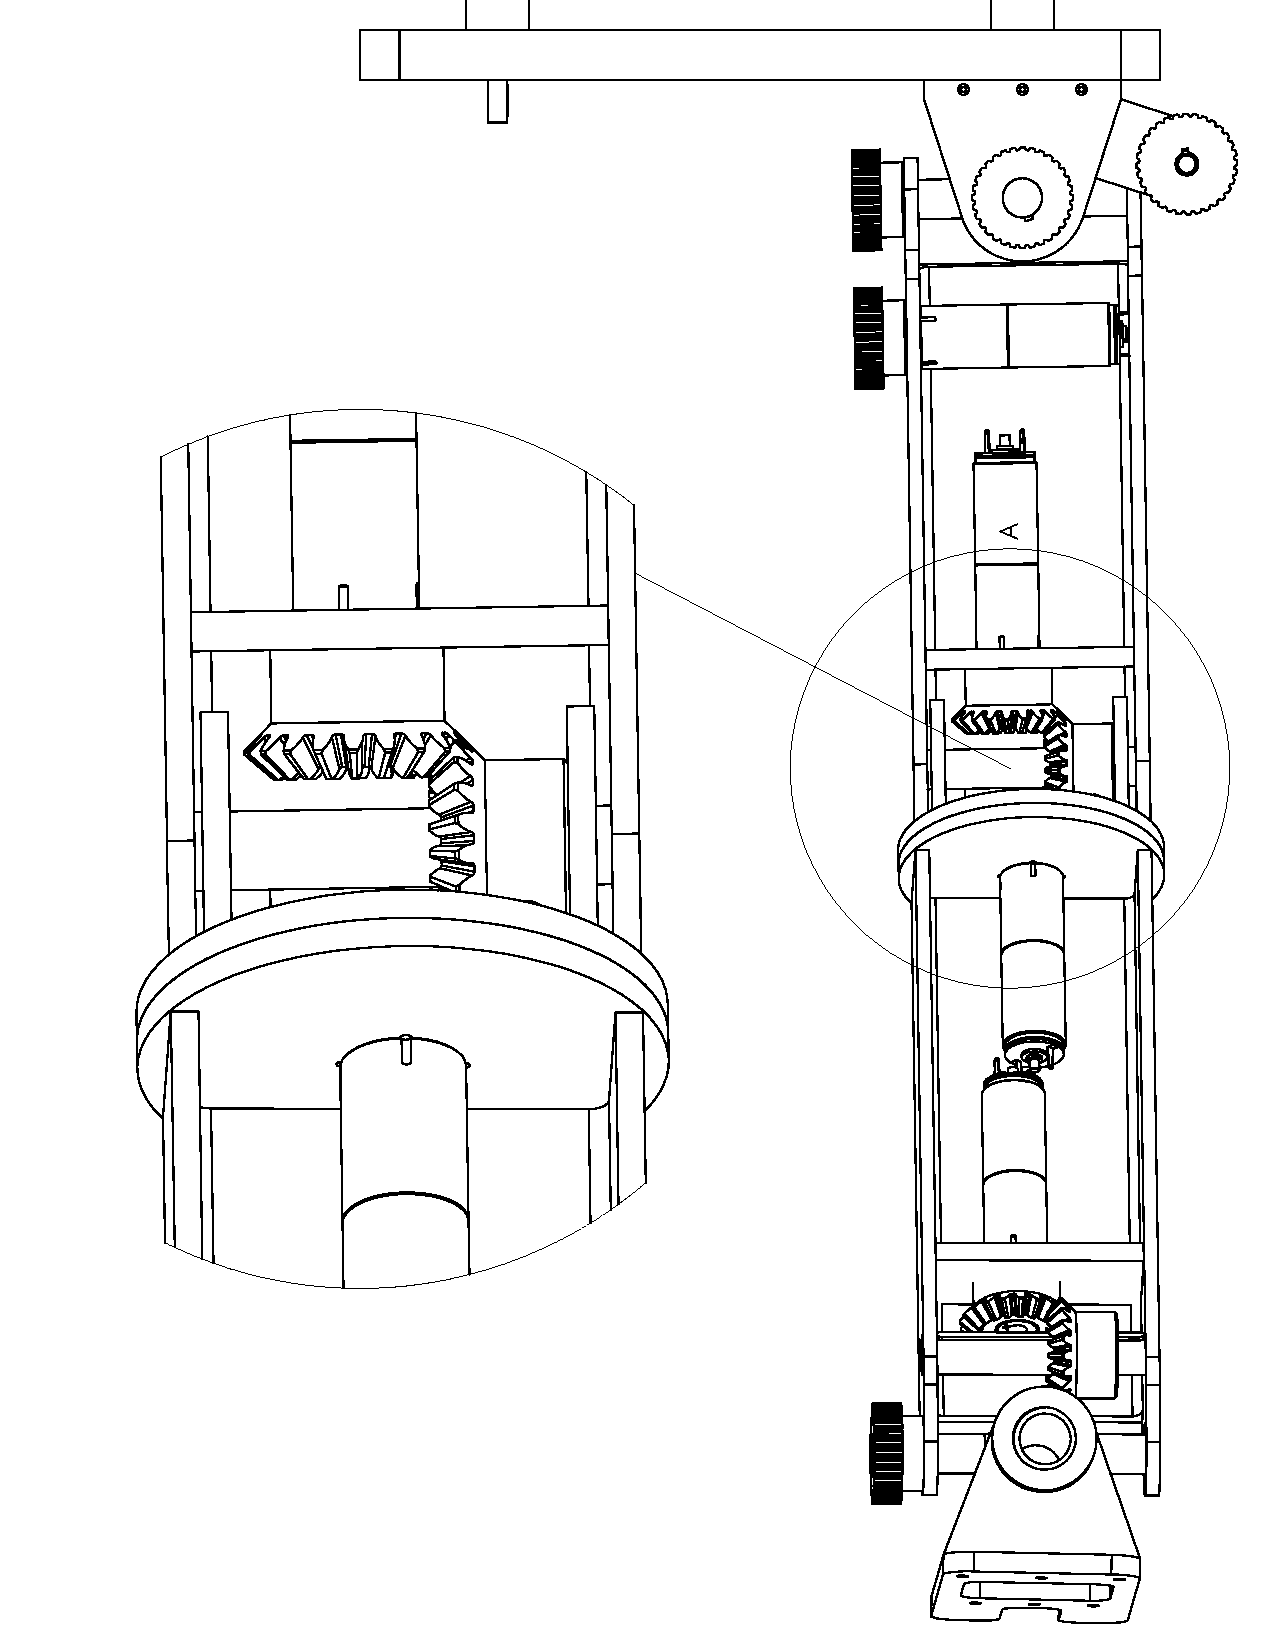
\includegraphics[scale=0.5]{fig/design/perpendicular.pdf}
	\end{center}
  \caption{Perpendicular mechanical coupling to shift weight distribution.}
\label{fig:miter}
\end{figure}

Mechanical coupling and power transmission are also used to design  intersecting axes of rotation. By using spur gears with a 1:1 reduction ratio, the output shaft of a drivetrain assembly can be positioned in a parallel offset (illustrated in Figure \ref{fig:spur}).

\begin{figure}[!h]	
	\begin{center}
    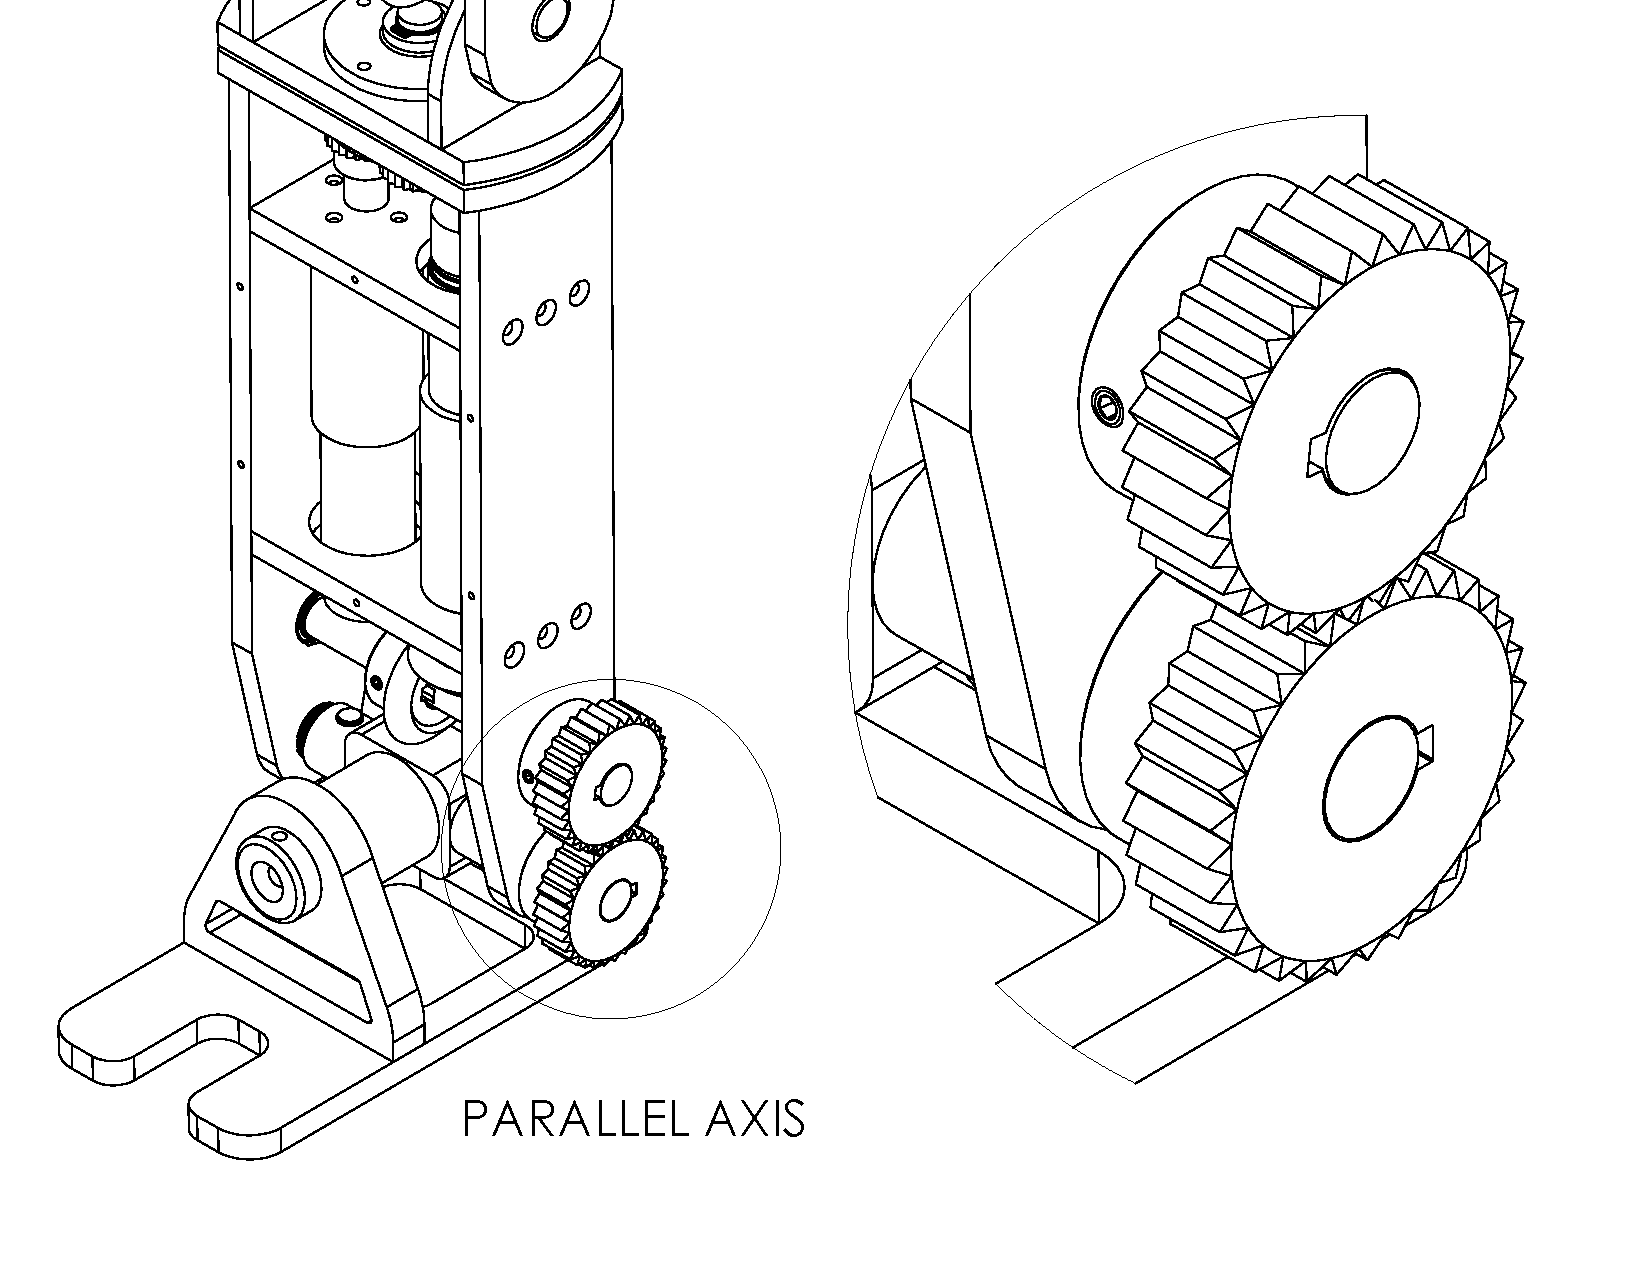
\includegraphics[scale=0.5]{fig/design/parallel.pdf}
	\end{center}
  \caption{Parallel mechanical coupling to allow intersection axis of rotation.}
\label{fig:spur}
\end{figure}

Shafts are frequently used to enable rotation between two link segments in the mechanical design. Ball bearings are common machine components which support the rotational movement of these shafts within a solid frame chassis. Traditional shielded ball bearings were selected for joints to support radial loads while permitting the rotation of a shaft on the inner ring (as illustrated in Figure \ref{fig:ballb}). The double shielded construction provides protection against debris from entering the bearing assembly without producing significant internal friction forces that are present in the case of sealed bearings. 

\begin{figure}[!h]
	\begin{center}
    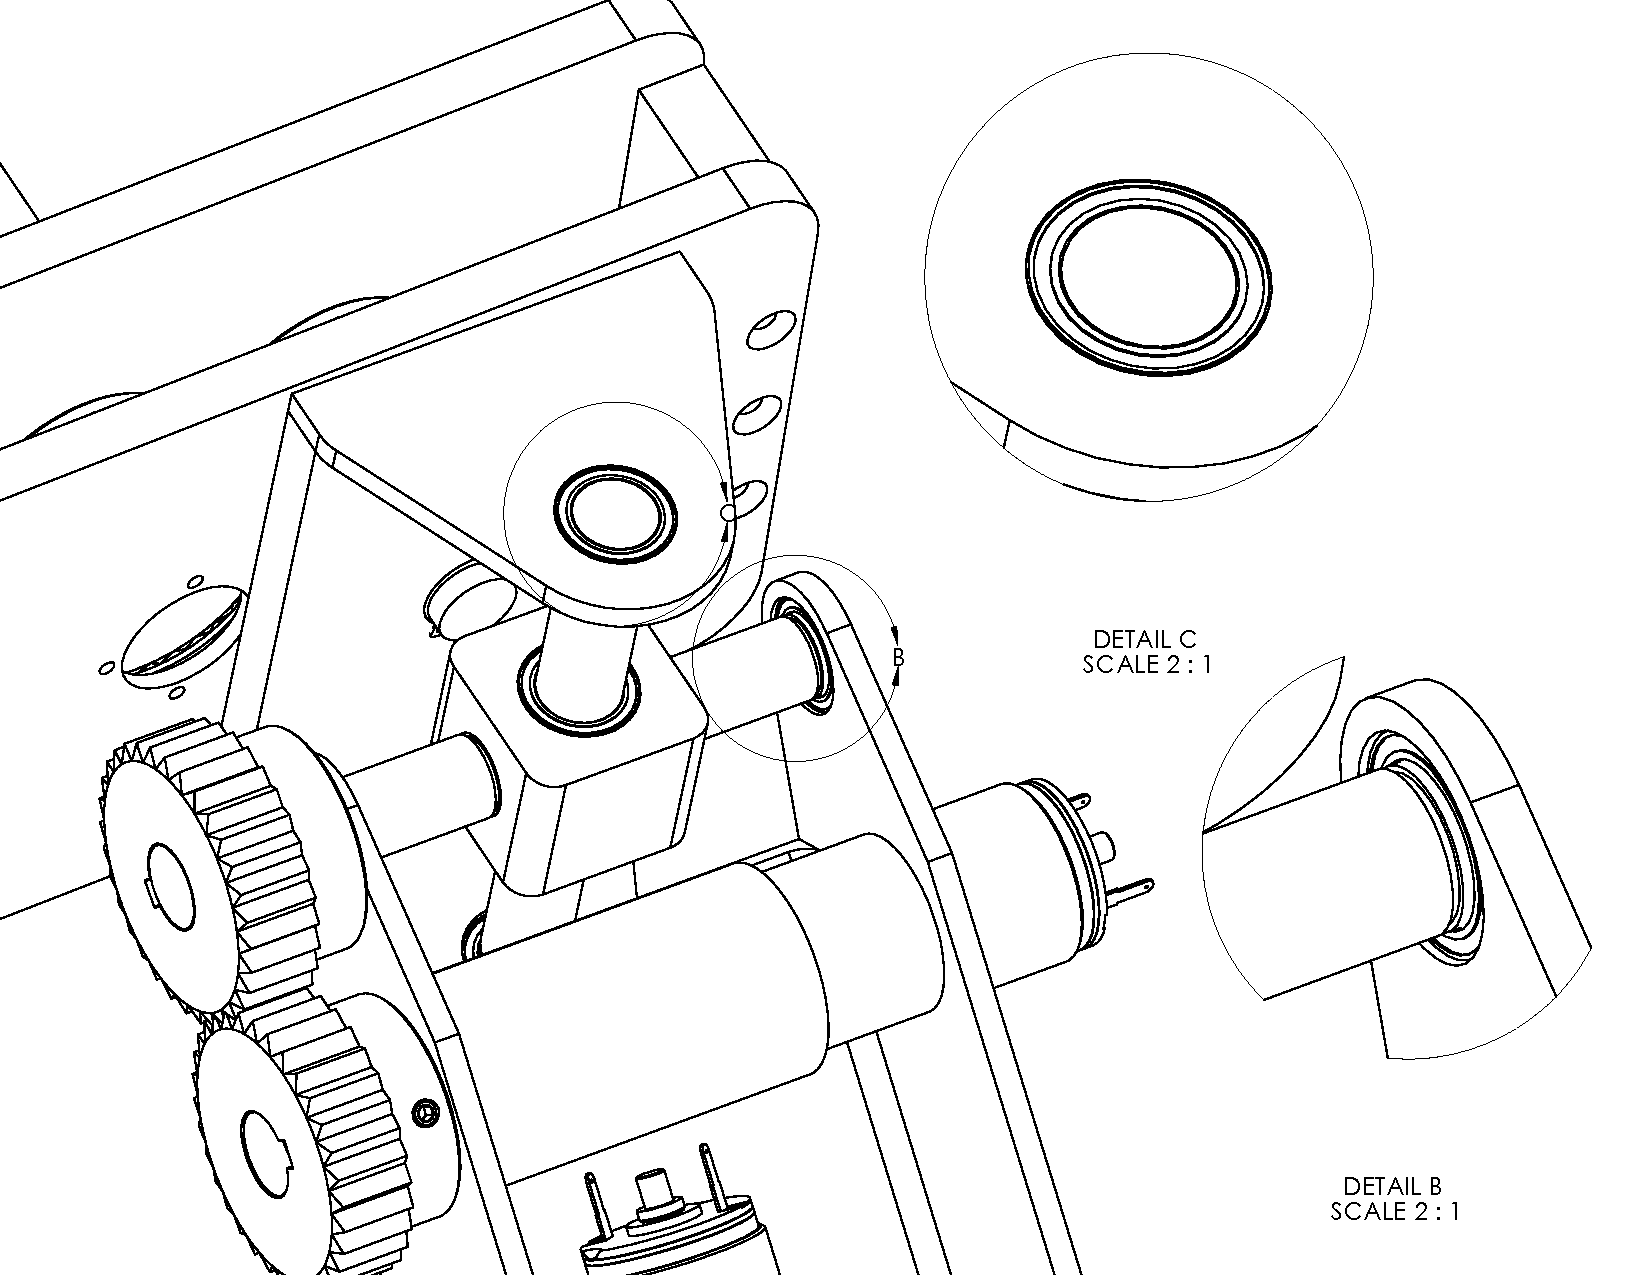
\includegraphics[scale=0.5]{fig/design/ballbearings.pdf}
	\end{center}
  \caption{Enabling rotational motion of shafts using double shielded ball bearings.}
\label{fig:ballb}
\end{figure}

For yaw joints which actuate along the vertical axis, the impact forces experienced during the gait cycle exert an axial load which is typically not supported by traditional ball bearings (would cause the inner ring to ``pop out''). Furthermore, these joints experience axial loads in one direction while the robot is standing on the ground but the load reverses direction if the robot is picked up by the torso. Therefore, bidirectional support for axial loads is required for the hip and ankle yaw joints. For these sections of the lower body, a combination of thrust and ball bearings are used to support radial and axial loads (as shown in Figure~\ref{fig:yawbearing}). 

\begin{figure}[!ht]
	\begin{center}
    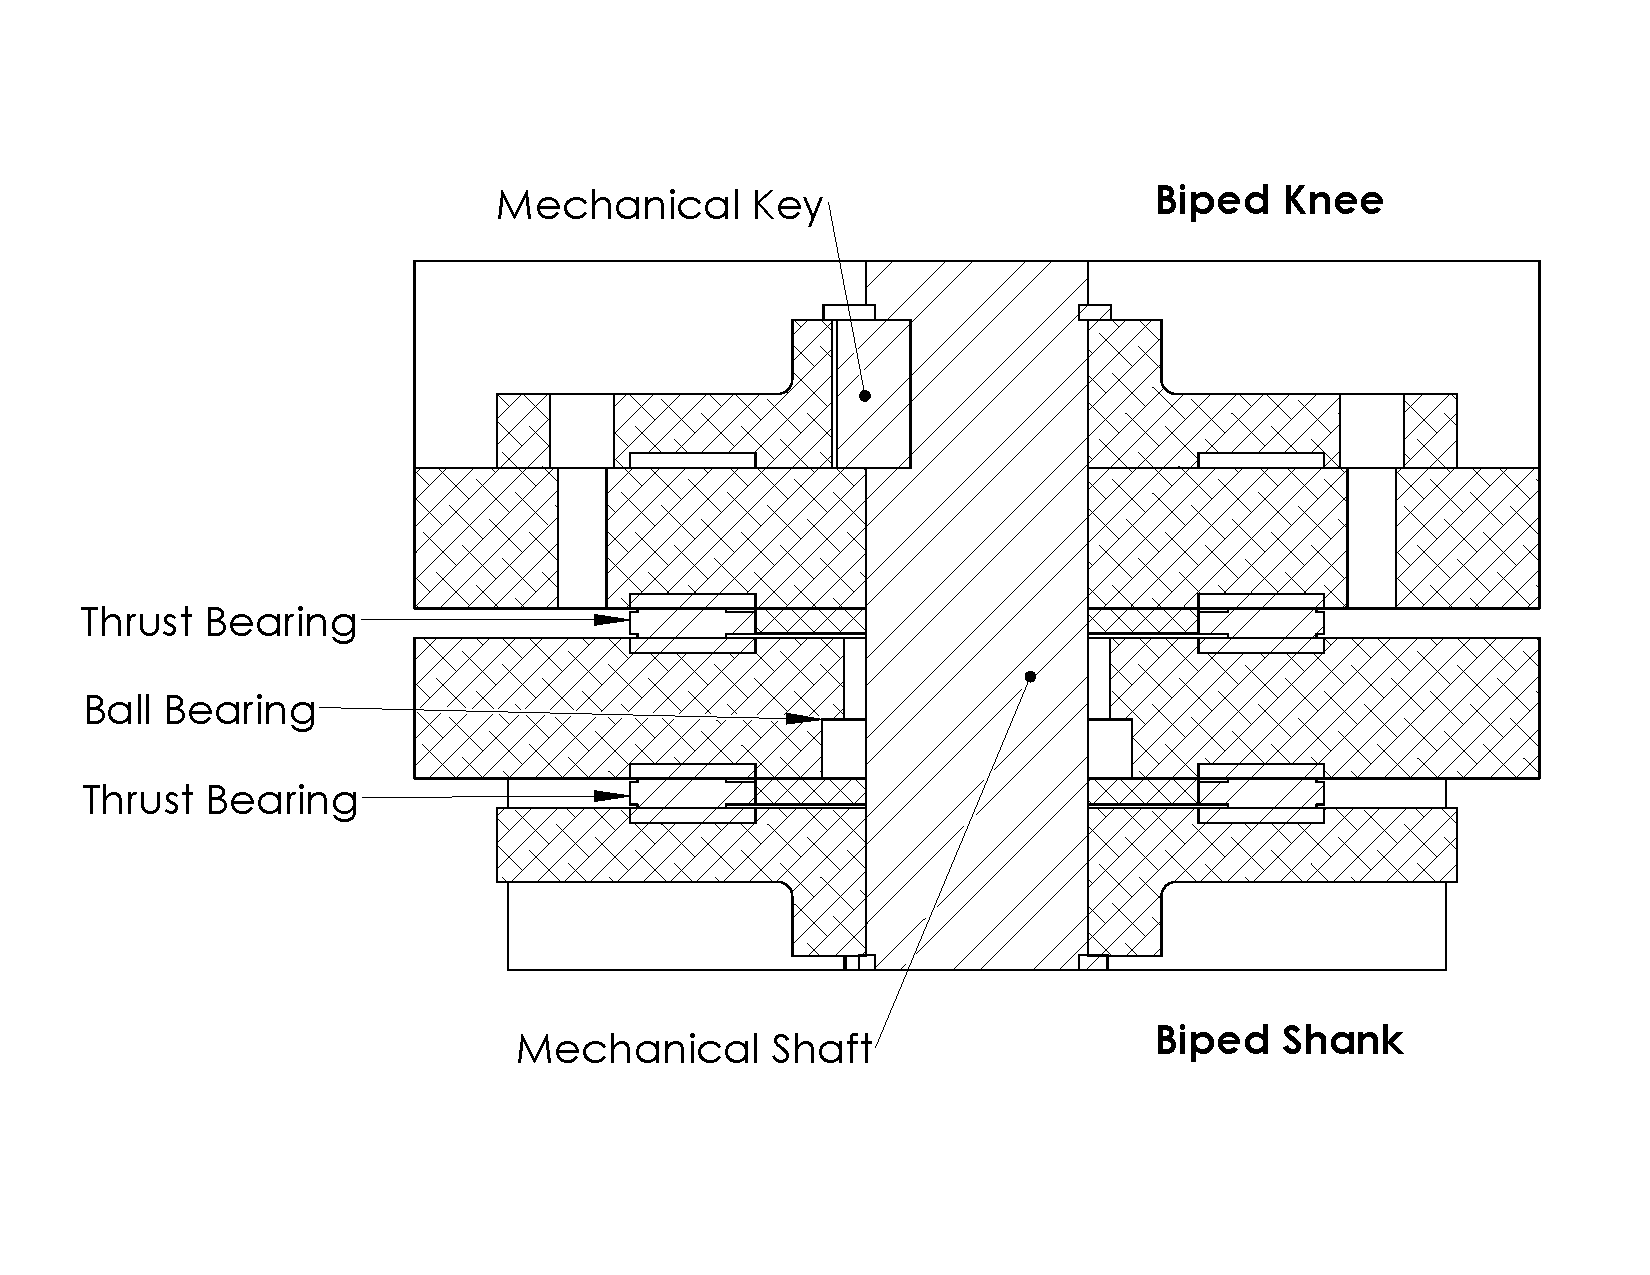
\includegraphics[trim = 5mm 34mm 5mm 25mm,clip,width=15cm]{fig/design/yawbearing.pdf}
	\end{center}
  \caption{A combination of thrust and ball bearings used for yaw joints to support radial and axial loading.}
\label{fig:yawbearing}
\end{figure}

The complete mechanical CAD drawings of the 14-DOF bipedal robot can be found in Appendix~\ref{app:bipedcad}. 

% subsubsection mechanical_power_transmission (end)

% section mechanical_design (end)

\section{Summary} % (fold)
\label{sec:design_summary}
The electromechanical design of the 14 DOF bipedal robot had two primary design objectives. The first was to produce enough mechanical power for the biped to achieve walking. The secondary design objective to keep the overall weight low and raise the COM improves the controllability of the final design. The initial design process started with basic dynamic modeling of the lower body. The forward and inverse dynamic models computed with the RNE algorithm provided a mathematical framework for estimating the torque requirements at each joint. 

Since the end goal is to develop a biped capable of human-like walking, a published dataset of motion captured human gait was used for the initial dynamic simulation. Using Matlab toolboxes, the kinematic constraints on each joint ($\q$, $\vec{\dot{q}}$, $\vec{\ddot{q}}$) were imposed on the dynamic model of the biped. A spring-damper contact model was used to generate an approximate ground reaction force experienced by the biped while walking. Finally, the initial joint torque and velocity demands under the estimated gait cycle were obtained through the dynamic simulations. 

These initial design specifications formed the basis for drivetrain selection. The primary design goal of producing enough mechanical power for bipedal locomotion was addressed by appropriately sizing motors to the specifications. A combination of DC motors and precision gearheads were evaluated by analyzing the torque-speed, power, efficiency and thermal characteristics. The selection process revealed that a set of high and low power configuration of drivetrain components would meet the specifications while minimizing the overall weight of the system. 

After the drivetrain configurations were established, the secondary design goal of minimizing the overall weight and raising the COM were addressed through the mechanical design of the chassis. A rough guideline for dimensioning the lower body segments (i.e. thigh, shank) was obtained through anthropometric dimensioning and the desired height of the lower body. Aluminum 5052 was selected as the material to construct the chassis frame due to its light weight, fatigue strength and machineability. The power transmission system (composed of shafts, bearings and gears) connecting the actuators to the linkages were strategically designed to raise the COM and support the loading during gait. 
% section discussion (end)

% chapter design (end)